\documentclass[preprint,12pt,authoryear]{elsarticle}

\usepackage[T1]{fontenc}
\usepackage{amsmath}
\usepackage{graphicx}
\usepackage{booktabs}
\usepackage{makecell}
\usepackage{tabularx}
\usepackage{array}
\usepackage{longtable}
\usepackage{microtype}
\usepackage{xcolor}
\usepackage{url}
\usepackage[hidelinks]{hyperref}
\usepackage[capitalise,noabbrev]{cleveref}
\pdfstringdefDisableCommands{\def\corref#1{}}
\emergencystretch=2em

% Generated by scripts/build.py -- do not edit.
\newcommand{\numAltAndroidMaxOffset}{6}
\newcommand{\numAltIosCells}{1{,}837}
\newcommand{\numAltIosHigh}{0}
\newcommand{\numAltIosLow}{-112}
\newcommand{\numAltIosMedian}{-46}
\newcommand{\numAltMax}{687}
\newcommand{\numAltMin}{-49}
\newcommand{\numAndroidBaroFraction}{100}
\newcommand{\numBadFixRate}{0.34}
\newcommand{\numBadFixes}{197}
\newcommand{\numBadHacc}{12.2}
\newcommand{\numBadHaccMax}{1{,}100}
\newcommand{\numBadMaxGap}{36.6}
\newcommand{\numBadRawFixes}{200}
\newcommand{\numBadSentinels}{9}
\newcommand{\numBadSpan}{586}
\newcommand{\numDeviceIds}{8}
\newcommand{\numDevices}{7}
\newcommand{\numDroppedSegments}{2}
\newcommand{\numEkfDegradedMedian}{440.4}
\newcommand{\numEkfDegradedN}{27}
\newcommand{\numEkfDegradedVMedian}{23.4}
\newcommand{\numEkfFullBad}{539}
\newcommand{\numEkfFullMaxOthers}{9.4}
\newcommand{\numEkfFullMedian}{4.1}
\newcommand{\numEkfFullN}{27}
\newcommand{\numEkfFullVMedian}{1.6}
\newcommand{\numExcludedRecordings}{4}
\newcommand{\numFixes}{197{,}522}
\newcommand{\numGravAfourteen}{9.806632}
\newcommand{\numGravAfourteenMedianDeficit}{73}
\newcommand{\numGravAfourteenPfiveDeficit}{22}
\newcommand{\numGravAfourteenPinned}{0.0}
\newcommand{\numGravAfourteenPninetyfiveDeficit}{156}
\newcommand{\numGravPixel}{9.810004}
\newcommand{\numGravRawPinnedMin}{100.0}
\newcommand{\numGravRawPinnedRecordings}{24}
\newcommand{\numGravSamsungApple}{9.806652}
\newcommand{\numGravTenHzPinnedMedian}{85}
\newcommand{\numHaccMax}{12.2}
\newcommand{\numHaccMin}{1.5}
\newcommand{\numHardIronCount}{20}
\newcommand{\numHardIronMax}{325}
\newcommand{\numHardIronMin}{67}
\newcommand{\numIosBaroFraction}{9}
\newcommand{\numLatMax}{42.07}
\newcommand{\numLatMin}{38.87}
\newcommand{\numLonMax}{72.11}
\newcommand{\numLonMin}{80.11}
\newcommand{\numMagIntensityMax}{240}
\newcommand{\numMagIntensityMin}{18}
\newcommand{\numMaxHours}{4.95}
\newcommand{\numMaxKm}{497.2}
\newcommand{\numMedianFixRate}{1.00}
\newcommand{\numMedianHacc}{2.5}
\newcommand{\numMedianHours}{1.74}
\newcommand{\numMedianKm}{141.8}
\newcommand{\numMedianSacc}{0.20}
\newcommand{\numMedianSpeed}{88}
\newcommand{\numMedianVacc}{2.0}
\newcommand{\numMinHours}{0.11}
\newcommand{\numMinKm}{1.1}
\newcommand{\numNoBaroHours}{8.8}
\newcommand{\numNoBaroRecordings}{2}
\newcommand{\numRawFirst}{2023-08}
\newcommand{\numRawGB}{22.2}
\newcommand{\numRawHours}{66.5}
\newcommand{\numRawLast}{2025-11}
\newcommand{\numRawNonEmpty}{28}
\newcommand{\numRawRecordings}{29}
\newcommand{\numRawRowsMillion}{219}
\newcommand{\numRbpfDegradedMedian}{817.7~km}
\newcommand{\numRbpfDegradedMissing}{2025-07-08\_14-12-53}
\newcommand{\numRbpfDegradedN}{26}
\newcommand{\numRbpfDegradedVMedian}{445.7}
\newcommand{\numRbpfFullMedian}{1.9}
\newcommand{\numRbpfFullN}{27}
\newcommand{\numRbpfFullVMedian}{1.6}
\newcommand{\numRows}{1{,}990{,}998}
\newcommand{\numSentinelTotal}{14}
\newcommand{\numSentinelTrajectories}{2}
\newcommand{\numSnrGravity}{0.13}
\newcommand{\numSnrGravityBest}{0.38}
\newcommand{\numSnrMagnetic}{0.01}
\newcommand{\numSnrMagneticBest}{0.04}
\newcommand{\numSplitRecordings}{1}
\newcommand{\numTotalHours}{55.3}
\newcommand{\numTotalKm}{4{,}338}
\newcommand{\numTrajectories}{27}
\newcommand{\numUkfDegradedMedian}{430.4}
\newcommand{\numUkfDegradedN}{27}
\newcommand{\numUkfDegradedVMedian}{24.0}
\newcommand{\numUkfFullBad}{543}
\newcommand{\numUkfFullMaxOthers}{9.3}
\newcommand{\numUkfFullMedian}{4.0}
\newcommand{\numUkfFullN}{27}
\newcommand{\numUkfFullVMedian}{1.6}
\newcommand{\numUsedRecordings}{25}
\newcommand{\numUtcNamed}{29}


% Visible placeholder for anything the authors still have to supply. Every use is listed in
% NOTES.md; a submission must not contain one.
\newcommand{\todo}[1]{\textbf{\textcolor{red}{[TODO: #1]}}}

\journal{Data in Brief}

\begin{document}

\begin{frontmatter}

\title{MEMS-Nav: \numTotalHours\texorpdfstring{~}{ }hours of synchronized smartphone inertial, GNSS, barometric and magnetic recordings from road vehicles for research on GNSS-degraded navigation}

\author[tu]{James Brodovsky\corref{cor1}}
\ead{jbrodovsky@temple.edu}
\author[tu]{Philip Dames}
\cortext[cor1]{Corresponding author.}
\affiliation[tu]{organization={Temple University}, addressline={[TODO: department]},
  city={Philadelphia}, state={PA}, postcode={19122}, country={USA}}

\begin{abstract}
Research on navigation without, or with degraded, satellite positioning needs long recordings from low-cost inertial sensors, because the errors that matter grow over minutes to hours rather than seconds. Most public navigation datasets are instead short, collected on a campus or in a city, and built around cameras or lidar. MEMS-Nav contains \numRawRecordings{} drives recorded with the Sensor Logger application on \numDevices{} smartphone models (Google Pixel, Samsung Galaxy and Apple iPhone) between \numRawFirst{} and \numRawLast{} in the north-eastern United States, mostly at highway speed. The raw release keeps every sensor stream at the rate the phone delivered it, typically about 100~Hz for the accelerometer, gyroscope, magnetometer, operating-system gravity and attitude, and about 1~Hz for GNSS. The processed release cuts the recordings at inertial dropouts into \numTrajectories{} synchronized trajectories at 10~Hz, totalling \numTotalHours~h and \numTotalKm~km (median \numMedianHours~h and \numMedianKm~km), with \numFixes{} GNSS fixes left at their native rate and never interpolated. Each trajectory ships with cropped relief, free-air gravity anomaly and magnetic anomaly grids. The data are described per device, per channel and per trajectory, together with three properties of phone sensors that matter to anyone attempting map-based aiding: the receiver's advertised accuracies, a gravity vector whose norm the operating system holds at a device constant, and a magnetometer dominated by the vehicle's own field. The open-source simulator strapdown-rs replays every trajectory and can withhold or corrupt the GNSS fixes, and reference baselines are reported for an extended Kalman filter, an unscented Kalman filter and a Rao--Blackwellized particle filter. With every fix, the two Kalman filters agree with the recorded GNSS track to a median horizontal RMSE of \numEkfFullMedian~m and \numUkfFullMedian~m. With one corrupted fix per minute, the median grows to \numEkfDegradedMedian~m and \numUkfDegradedMedian~m. The reference position is the phone's own GNSS solution, not an independent ground truth.

\end{abstract}

\begin{keyword}
Inertial navigation \sep MEMS inertial measurement unit \sep Smartphone sensors \sep GNSS degradation \sep Sensor fusion \sep Kalman filter \sep Geophysical navigation \sep Magnetometer
\end{keyword}

\end{frontmatter}

\section*{Specifications table}
\label{sec:specifications}

\begin{longtable}{@{}>{\raggedright\arraybackslash}p{0.25\linewidth}>{\raggedright\arraybackslash}p{0.70\linewidth}@{}}
\toprule
Subject & Engineering \todo{choose from the Data in Brief subject list} \\
\midrule
Specific subject area & Inertial and satellite navigation with consumer-grade MEMS sensors; sensor fusion and state estimation under degraded or denied GNSS; geophysical (gravity and magnetic) map-aided navigation. \\
\midrule
Type of data & Time series in CSV tables (raw and processed); gridded map tiles in NetCDF; JSON segmentation manifest; TOML scenario configurations; tables and figures. \\
\midrule
Data collection & Smartphones running the Sensor Logger application \citep{sensorlogger} recorded the accelerometer, gyroscope, magnetometer, barometer, the operating system's fused gravity and attitude estimates, and GNSS fixes during road drives. The \numDevices{} phone models used were Google Pixel 6a, Pixel 9 Pro and Pixel 9 Pro XL; Samsung SM-S921U and SM-A146U; and Apple iPhone 12 mini and iPhone 13 mini. The phones were \todo{describe placement and mounting in the vehicle, and the vehicles used}. Recordings were resampled to 10~Hz, split at inertial dropouts longer than 5~s, and accompanied by map tiles from the Generic Mapping Tools remote datasets \citep{wessel2019gmt}, with the open-source analysis package distributed with strapdown-rs \citep{strapdown-rs}. \\
\midrule
Data source location & Public roads in the north-eastern United States, within latitudes \numLatMin--\numLatMax\,\textdegree{}N and longitudes \numLonMax--\numLonMin\,\textdegree{}W. Data were processed at Temple University, Philadelphia, Pennsylvania, USA. \\
\midrule
Data accessibility & Repository name: Zenodo \newline Data identification number: \todo{new Zenodo DOI} \newline Direct URL to data: \todo{https://doi.org/new Zenodo DOI} \newline Instructions for accessing these data: open access, no registration. The processing and replay software is available at \url{https://github.com/jbrodovsky/strapdown-rs}. \\
\midrule
Related research article & J.~Brodovsky, P.~Dames, Navigation in GNSS-denied environments using MEMS-grade sensors and geophysical anomalies: a UKF approach, in: Proceedings of the 2026 International Technical Meeting of the Institute of Navigation, Anaheim, California, 2026, pp.~155--164. \url{https://doi.org/10.33012/2026.20508} \\
\bottomrule
\end{longtable}
\addtocounter{table}{-1}

\section*{Value of the data}
\label{sec:value}

\begin{itemize}
\item \textbf{Duration and distance at consumer grade.} The \numTrajectories{} trajectories cover \numTotalHours~h and \numTotalKm~km of driving, up to \numMaxHours~h and \numMaxKm~km in one trajectory. Inertial error over GNSS outages of minutes to hours can therefore be studied on consumer MEMS hardware, rather than inferred from the seconds-long sequences of most robotics datasets.
\item \textbf{Several devices and both mobile platforms.} Seven phone models from three manufacturers, on Android and iOS, were recorded with the same application and are processed into one column layout. Methods can be compared across inertial sensors, sampling rates and receivers, and their sensitivity to the device can be measured.
\item \textbf{Raw streams kept beside the processed files.} The raw recordings keep each sensor at its delivered rate (about 100~Hz for the inertial sensors on most devices), together with the uncalibrated accelerometer, gyroscope and magnetometer streams where the phone provided them. Users can therefore choose their own resampling, synchronization and calibration instead of inheriting ours.
\item \textbf{Ready for controlled GNSS degradation.} Every trajectory runs unmodified in the open-source simulator strapdown-rs \citep{strapdown-rs}. The simulator can withhold GNSS fixes on a schedule and corrupt them with correlated noise, slow drift or step offsets, all from a seeded configuration file. One recording can therefore be replayed under many repeatable outage and spoofing scenarios, and the baselines reported here give a starting point for comparing new methods.
\item \textbf{Documented sensor caveats for map-based aiding.} Cropped relief, gravity-anomaly and magnetic-anomaly grids are supplied for every trajectory. We also document that the phones' gravity vector carries no gravity-anomaly information and that their magnetometers are dominated by the vehicle's field. This saves geophysical and magnetic navigation studies from basing an aiding experiment on channels that cannot support it.
\end{itemize}

\section{Background}
\label{sec:background}

An inertial navigation system integrates angular rate and specific force to propagate position, velocity and attitude, and its error grows without bound unless an external measurement corrects it \citep{groves}. In most vehicles that correction is GNSS. Interference, spoofing and plain unavailability can remove or corrupt it \citep{9112619}, which has driven interest in alternative position sources such as gravity and magnetic anomaly maps \citep{canciani2016absolute,canciani2017airborne,gravnav}. Developing and comparing such methods requires recordings in which the inertial error has time to grow. With consumer MEMS sensors that means drives of tens of minutes to hours, and for map-based aiding it also means distances long enough to cross map features. The public grids used here have cells of 1 arc-minute for the free-air gravity anomaly and 3 arc-minutes for the magnetic anomaly, about 1.9 and 5.6~km \citep{SANDWELL20211059,wdmam}.

Existing datasets fit this need poorly. Vehicle and robot datasets such as KITTI \citep{kitti}, Oxford RobotCar \citep{oxford-robotcar}, the Ford campus set \citep{ford-campus}, the DARPA Urban Challenge set \citep{mit-darpa}, KAIST Urban \citep{kaist-urban} and NCLT \citep{nclt} pair navigation-grade inertial or GNSS/INS references with cameras and lidar, and they are recorded on campuses or in cities. Aerial and handheld visual--inertial sets \citep{burri2016euroc,tum-vi,uzh-fpv,nguyen2022ntu,newer-college} last minutes. Smartphone datasets exist, but they target other problems: raw GNSS measurements for precise positioning \citep{fu2020android}, or pedestrian inertial odometry \citep{herath2020ronin}. Inertial datasets for autonomous platforms \citep{ansfl,yampolsky2024multiple} are built around dedicated inertial units. To our knowledge, no public dataset combines hours-long road drives, consumer phone inertial sensors from several manufacturers, barometer and magnetometer streams, and a ready-made way to impose controlled GNSS degradation.

An earlier version of MEMS-Nav was released as a preprint and a GitHub repository with 17 trajectories at about 1~Hz \citep{memsnav-preprint}, and parts of it were used to evaluate anomaly-aided filters \citep{anom-ukf,anom-pf}. This article supersedes that release. It adds the raw recordings at their delivered rates, \numTrajectories{} trajectories in place of 17, a 10~Hz processed form, per-device and per-channel documentation, map tiles for every trajectory, reference baselines under a specified degradation scenario, and a characterization of the phone channels that explains why they bring no measurable benefit when used as anomaly measurements \citep{brodovsky2026dissertation}.

\section{Data description}
\label{sec:description}

The dataset has three tiers: the raw recordings exactly as the phones exported them, the processed trajectories that most users will start from, and the map tiles and benchmark material that accompany the processed trajectories. \Cref{tab:devices} summarizes the recordings by device and \Cref{fig:tracks} shows where they were made.

\subsection{Repository layout}
\label{sec:layout}

The Zenodo record \todo{new Zenodo DOI} is organized as follows. \todo{confirm the final directory names once the record is assembled; the layout below is the one proposed for it.}

\begin{itemize}
\item \texttt{raw/<recording>/}: one directory per recording, named by its UTC start time as \texttt{YYYY-MM-DD\_hh-mm-ss}. All \numUtcNamed{} directory names match the epoch timestamp stored in their \texttt{Metadata.csv}. Each directory holds the Sensor Logger CSV exports (\Cref{sec:raw}).
\item \texttt{processed/<trajectory>.csv}: the \numTrajectories{} synchronized 10~Hz trajectories (\Cref{sec:processed}). A trajectory cut from a recording that had to be split carries a suffix \texttt{\_A}, \texttt{\_B}, \ldots{} in time order.
\item \texttt{processed/segments.json}: the segmentation manifest. It has one entry per recording or segment, giving the source recording, the start and end time in seconds from the start of the recording, the row count, and whether the segment was kept or why it was rejected.
\item \texttt{maps/<trajectory>\_\{relief,gravity,magnetic\}.nc}: map tiles cropped to each trajectory (\Cref{sec:maps}).
\item \texttt{benchmark/}: the scenario configurations and the per-trajectory error summaries behind \Cref{tab:benchmark}.
\end{itemize}

\begin{table}[t]
\centering
\caption{Recordings by device, as identified in each recording's \texttt{Metadata.csv}. \emph{Rec.}\ counts raw recordings and \emph{Traj.}\ counts processed trajectories; hours and distance are those of the processed trajectories. \emph{GNSS file} is the raw file that the processed GNSS columns are taken from: \texttt{LocationGps} is Android's GNSS-only provider and \texttt{Location} is the platform's fused location service.}
\label{tab:devices}
\small
\begin{tabular}{llrrrrl}
\toprule
Device (as logged) & OS & Rec. & Traj. & Hours & km & GNSS file \\
\midrule
Pixel 6a & Android & 5 & 5 & 9.4 & 593 & \texttt{LocationGps} \\
SM-S921U & Android & 2 & 2 & 3.0 & 228 & \texttt{Location} \\
Pixel 9 Pro & Android & 12 & 13 & 26.9 & 2{,}159 & \texttt{LocationGps} \\
SM-A146U & Android & 2 & 1 & 0.2 & 13 & \texttt{Location} \\
Pixel 9 Pro XL & Android & 2 & 2 & 3.7 & 294 & \texttt{LocationGps} \\
iPhone 12 mini & iOS & 5 & 3 & 10.3 & 956 & \texttt{Location} \\
iPhone 13 mini & iOS & 1 & 1 & 1.8 & 96 & \texttt{Location} \\
\midrule
Total & & 29 & 27 & 55.3 & 4{,}338 & \\
\bottomrule
\end{tabular}

\end{table}

\begin{figure}[t]
\centering
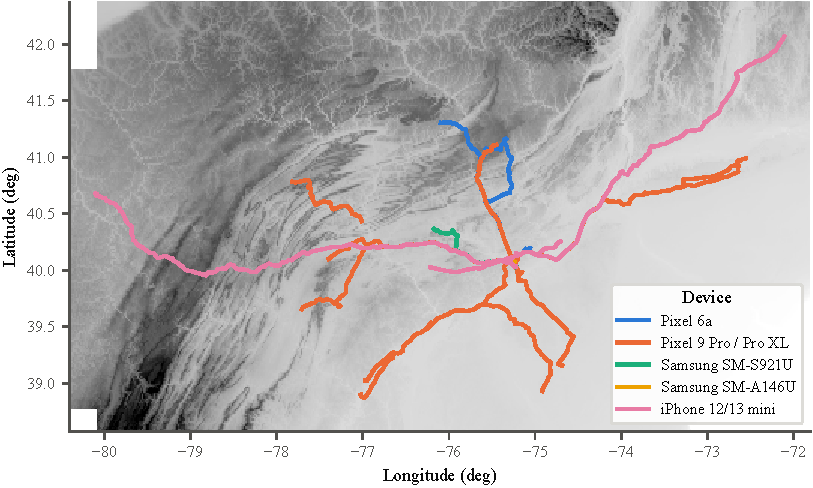
\includegraphics[width=\linewidth]{figures/fig_tracks.pdf}
\caption{GNSS tracks of the \numTrajectories{} processed trajectories, colored by device family, over the 15 arc-second relief tiles that accompany them (darker is higher). The single Samsung SM-A146U trajectory is short and lies under other tracks near 40.1\textdegree{}N, 75.3\textdegree{}W.}
\label{fig:tracks}
\end{figure}

\subsection{Raw recordings}
\label{sec:raw}

There are \numRawRecordings{} raw recordings, made between \numRawFirst{} and \numRawLast{} with Sensor Logger versions 1.18.0 to 1.48.0 \citep{sensorlogger}. Together they hold \numRawGB~GB in about \numRawRowsMillion{} million rows and span \numRawHours~h of wall-clock time. One recording (\texttt{2025-06-13\_14-55-15}) contains no sensor data. Every sensor file has the columns \texttt{time}, the UTC epoch time in nanoseconds, and \texttt{seconds\_elapsed}, the time since the recording started, followed by its measured quantities. Three-axis sensors give \texttt{x}, \texttt{y} and \texttt{z} in the phone's body frame as reported by the operating system. \texttt{Metadata.csv} records the device model, platform, application version, the list of enabled sensors, their requested sampling interval in milliseconds, and whether Sensor Logger's cross-platform unit standardization was on.

The files present depend on the platform and the application version. All recordings with data have \texttt{Gyroscope}, \texttt{Accelerometer}, \texttt{Gravity}, \texttt{Magnetometer}, \texttt{Orientation} and \texttt{Location}. Android recordings add \texttt{TotalAcceleration} (specific force including gravity). Recordings from 2025 onward add \texttt{GyroscopeUncalibrated}, \texttt{AccelerometerUncalibrated}, \texttt{MagnetometerUncalibrated} and \texttt{Compass}. Pixel recordings add the separate GNSS (\texttt{LocationGps}) and network (\texttt{LocationNetwork}) location providers, and Pixel 9 Pro recordings also add \texttt{GameOrientation} and \texttt{GeomagneticOrientation}. On both platforms \texttt{Accelerometer} is linear acceleration, with gravity removed. \numNoBaroRecordings{} iPhone recordings (\numNoBaroHours~h) have no barometer data and are released in raw form only. \Cref{tab:channels} lists the median sampling rate of each channel by device family, measured from the timestamps.

\begin{table}[t]
\centering
\caption{Sensor channels. Rates are the median, over the recordings of each device family that enter the processed set, of each recording's median sampling rate (Hz) in the raw files; every channel is resampled to 10~Hz in the processed files. Sensor Logger requested a 10~ms interval for all inertial channels and left the barometer and location at their defaults. (a)~On iOS, where there is no \texttt{TotalAcceleration}, specific force is formed as \texttt{Accelerometer} plus \texttt{Gravity}. (b)~\texttt{Location} where \texttt{LocationGps} is absent (\Cref{tab:devices}). Processed column names are abbreviated; \Cref{sec:processed} lists them in full with their units.}
\label{tab:channels}
\footnotesize
\setlength{\tabcolsep}{2.5pt}
\begin{tabular}{llllrrrrr}
\toprule
Channel & Raw file & Columns & Unit & \rotatebox{90}{Pixel 6a} & \rotatebox{90}{Pixel 9 Pro / Pro XL} & \rotatebox{90}{Samsung SM-S921U} & \rotatebox{90}{Samsung SM-A146U} & \rotatebox{90}{iPhone 12/13 mini} \\
\midrule
Specific force & \texttt{TotalAcceleration}\textsuperscript{a} & \texttt{acc\_*} & m\,s\(^{-2}\) & 56 & 100 & 60 & 100 & 101 \\
Angular rate & \texttt{Gyroscope} & \texttt{gyro\_*} & rad\,s\(^{-1}\) & 56 & 100 & 60 & 100 & 101 \\
Magnetic field & \texttt{Magnetometer} & \texttt{mag\_*} & \(\mu\)T & 100 & 100 & 100 & 100 & 101 \\
Gravity (fused) & \texttt{Gravity} & \texttt{grav\_*} & m\,s\(^{-2}\) & 56 & 100 & 100 & 100 & 101 \\
Attitude (fused) & \texttt{Orientation} & \texttt{q*}, \texttt{roll}, \ldots & --, rad & 56 & 100 & 100 & 100 & 101 \\
Pressure & \texttt{Barometer} & \texttt{pressure}, \ldots & hPa, m & 50 & 40 & 25 & 10 & 1 \\
GNSS fix & \texttt{LocationGps}\textsuperscript{b} & \texttt{latitude}, \ldots & see text & 1 & 1 & 1 & 1 & 1 \\
\bottomrule
\end{tabular}

\end{table}

\subsection{Processed trajectories}
\label{sec:processed}

The \numTrajectories{} processed trajectories hold \numRows{} rows at 10~Hz. \Cref{tab:trajectories} lists them. They last from \numMinHours~h to \numMaxHours~h and cover \numMinKm~km to \numMaxKm~km, for \numTotalHours~h and \numTotalKm~km in total. The median GNSS speed is \numMedianSpeed~km/h, so most of the driving is on highways. Each file has the following columns.
\begin{itemize}
\item \texttt{time}: ISO 8601 timestamp in UTC, at the start of each 0.1~s bin.
\item \texttt{latitude}, \texttt{longitude} (degrees, WGS84), \texttt{altitude} (m, as reported by the location service), \texttt{speed} (m/s), \texttt{bearing} (degrees from north), and the receiver's reported \texttt{horizontalAccuracy} (m), \texttt{verticalAccuracy} (m), \texttt{speedAccuracy} (m/s) and \texttt{bearingAccuracy} (degrees). These columns are filled only in rows that contain a GNSS fix and are empty elsewhere.
\item \texttt{acc\_x}, \texttt{acc\_y}, \texttt{acc\_z}: specific force in the body frame (m/s\(^2\)), including gravity, so that a phone at rest reads about \(+9.8\)~m/s\(^2\) along its upward axis.
\item \texttt{gyro\_x}, \texttt{gyro\_y}, \texttt{gyro\_z}: angular rate (rad/s), as calibrated by the operating system.
\item \texttt{mag\_x}, \texttt{mag\_y}, \texttt{mag\_z}: magnetic flux density (\(\mu\)T), with the operating system's hard-iron correction applied (\Cref{sec:magnetometer}).
\item \texttt{grav\_x}, \texttt{grav\_y}, \texttt{grav\_z}: the operating system's fused gravity estimate (m/s\(^2\); \Cref{sec:gravity}).
\item \texttt{qw}, \texttt{qx}, \texttt{qy}, \texttt{qz} and \texttt{roll}, \texttt{pitch}, \texttt{yaw} (rad): the operating system's fused attitude.
\item \texttt{pressure} (hPa) and \texttt{relativeAltitude} (m, change since the recording began, derived from pressure).
\end{itemize}
The GNSS columns hold \numFixes{} fixes, a median of \numMedianFixRate{} fixes per second per trajectory, and they are never interpolated: in about nine rows out of ten they are empty. The inertial columns are complete in every row. iOS phones deliver pressure at about 1~Hz, so on those trajectories only a median of \numIosBaroFraction\% of rows carry a pressure value.

\begin{table}[p]
\centering
\caption{The processed trajectories. \emph{Speed} is the median GNSS speed, \emph{Fixes} the number of rows with a GNSS fix, and \emph{Fix rate} the fixes per second of trajectory. \(\sigma_h\), \(\sigma_v\) and \(\sigma_s\) are the medians of the receiver's reported horizontal, vertical and speed accuracy over those fixes. Distance is the summed great-circle distance between successive fixes.}
\label{tab:trajectories}
\scriptsize
\setlength{\tabcolsep}{3pt}
\begin{tabular}{llrrrrrrrr}
\toprule
Trajectory & Device & h & km & \makecell{Speed\\(km/h)} & Fixes & \makecell{Fix\\rate (Hz)} & \makecell{\(\sigma_h\)\\(m)} & \makecell{\(\sigma_v\)\\(m)} & \makecell{\(\sigma_s\)\\(m/s)} \\
\midrule
2023-08-04\_21-47-58 & Pixel 6a & 2.45 & 158.3 & 87 & 8{,}034 & 0.91 & 2.0 & 2.5 & 0.18 \\
2023-08-06\_14-48-05 & Pixel 6a & 2.48 & 169.1 & 77 & 8{,}920 & 1.00 & 2.0 & 2.4 & 0.17 \\
2023-08-09\_12-47-42 & Pixel 6a & 1.45 & 32.1 & 3 & 5{,}174 & 0.99 & 2.6 & 3.1 & 0.23 \\
2023-08-09\_16-37-41 & Pixel 6a & 0.72 & 41.0 & 63 & 2{,}579 & 1.00 & 2.2 & 2.7 & 0.20 \\
2024-06-20\_16-55-50 & Pixel 6a & 2.34 & 192.3 & 99 & 8{,}391 & 1.00 & 7.8 & 3.0 & 0.23 \\
2025-03-01\_15-04-26 & SM-S921U & 1.51 & 114.2 & 84 & 5{,}457 & 1.00 & 3.8 & 1.3 & 0.08 \\
2025-03-01\_16-46-39 & SM-S921U & 1.49 & 113.6 & 83 & 5{,}386 & 1.00 & 3.8 & 1.3 & 0.08 \\
2025-06-11\_20-34-24\_A & Pixel 9 Pro & 0.11 & 2.1 & 16 & 411 & 1.00 & 6.6 & 3.0 & 0.46 \\
2025-06-14\_21-17-02 & SM-A146U & 0.16 & 12.7 & 2 & 197 & 0.34 & 12.2 & 0.7 & 0.39 \\
2025-06-18\_15-09-25 & Pixel 9 Pro XL & 1.48 & 148.9 & 111 & 5{,}248 & 0.98 & 8.2 & 3.0 & 0.38 \\
2025-06-18\_16-52-32 & Pixel 9 Pro XL & 2.20 & 144.9 & 74 & 7{,}916 & 1.00 & 5.1 & 2.0 & 0.20 \\
2025-06-27\_11-54-35 & iPhone 12 mini & 4.95 & 402.3 & 99 & 17{,}767 & 1.00 & 10.0 & 19.0 & 0.20 \\
2025-07-04\_17-24-46 & Pixel 9 Pro & 1.74 & 137.4 & 94 & 6{,}227 & 0.99 & 6.6 & 2.0 & 0.25 \\
2025-07-05\_20-59-22 & Pixel 9 Pro & 2.51 & 138.5 & 55 & 9{,}017 & 1.00 & 7.1 & 3.0 & 0.31 \\
2025-07-08\_14-12-53 & iPhone 13 mini & 1.85 & 96.2 & 55 & 6{,}658 & 1.00 & 2.5 & 3.0 & 1.56 \\
2025-07-11\_13-33-16 & Pixel 9 Pro & 1.66 & 136.2 & 98 & 5{,}961 & 1.00 & 1.5 & 1.0 & 0.12 \\
2025-07-18\_23-13-43 & Pixel 9 Pro & 1.55 & 152.1 & 109 & 5{,}526 & 0.99 & 1.5 & 1.0 & 0.13 \\
2025-07-31\_23-36-03 & Pixel 9 Pro & 3.74 & 304.6 & 88 & 13{,}450 & 1.00 & 1.5 & 1.0 & 0.13 \\
2025-08-03\_18-15-59 & Pixel 9 Pro & 4.14 & 298.2 & 84 & 14{,}892 & 1.00 & 1.5 & 1.0 & 0.14 \\
2025-09-26\_19-03-38 & iPhone 12 mini & 4.59 & 497.2 & 123 & 16{,}505 & 1.00 & 5.0 & 9.5 & 0.20 \\
2025-09-27\_12-54-35 & Pixel 9 Pro & 2.26 & 213.0 & 109 & 8{,}136 & 1.00 & 2.0 & 1.0 & 0.14 \\
2025-09-27\_18-10-16 & iPhone 12 mini & 0.76 & 56.3 & 89 & 2{,}731 & 1.00 & 10.0 & 19.0 & 0.20 \\
2025-09-28\_20-23-16 & Pixel 9 Pro & 3.33 & 286.3 & 99 & 11{,}996 & 1.00 & 2.0 & 1.0 & 0.13 \\
2025-11-09\_17-34-01\_A & Pixel 9 Pro & 1.07 & 108.0 & 106 & 3{,}854 & 1.00 & 1.5 & 1.0 & 0.12 \\
2025-11-09\_17-34-01\_B & Pixel 9 Pro & 0.16 & 1.1 & 0 & 559 & 1.00 & 2.0 & 1.0 & 0.01 \\
2025-11-09\_17-34-01\_C & Pixel 9 Pro & 1.40 & 141.8 & 115 & 5{,}020 & 1.00 & 2.0 & 1.0 & 0.31 \\
2025-11-16\_16-08-14 & Pixel 9 Pro & 3.23 & 239.1 & 90 & 11{,}510 & 0.99 & 2.0 & 1.0 & 0.14 \\
\midrule
Total & & 55.3 & 4{,}338 & & 197{,}522 & & & & \\
Median & & 1.74 & 141.8 & 88 & 6{,}227 & 1.00 & 2.5 & 2.0 & 0.20 \\
\bottomrule
\end{tabular}

\end{table}

\subsection{Map tiles}
\label{sec:maps}

Each processed trajectory comes with three NetCDF grids cropped to its padded bounding box. Each grid has variables \texttt{lat}, \texttt{lon} (degrees) and \texttt{z}: relief at 15 arc-seconds (m; SRTM15+, \citealp{tozer2019srtm15}), free-air gravity anomaly at 1 arc-minute (mGal; \citealp{SANDWELL20211059}) and magnetic anomaly at 3 arc-minutes (nT; WDMAM, \citealp{wdmam}). They were fetched through the Generic Mapping Tools remote datasets \citep{wessel2019gmt}, are provided for convenience, and remain subject to their originators' terms.

\section{Experimental design, materials and methods}
\label{sec:methods}

\subsection{Collection}
\label{sec:collection}

The drives were recorded by the authors and by volunteers (see Acknowledgements) on public roads. The phones ran Sensor Logger \citep{sensorlogger} with the accelerometer, gyroscope, magnetometer, gravity, orientation and barometer sensors enabled, together with location and, where offered, the uncalibrated and compass streams. Every inertial channel was requested at a 10~ms interval. The barometer and location were left at the application's default, which \texttt{Metadata.csv} records as an interval of 0. The phones were \todo{state where and how the phones were held in the vehicle (mount, cradle, cup holder, loose), whether the mount changed during a drive, and which vehicles were used}. \todo{confirm that no additional hardware and no external reference receiver were used}. \Cref{tab:devices} lists the devices; \Cref{tab:channels} gives the rates the phones actually delivered, which fall short of the request on some devices (about 56~Hz for the Pixel 6a's inertial channels and about 60~Hz for the Samsung SM-S921U's gyroscope).

\subsection{Processing}
\label{sec:processing}

The raw recordings were converted to the processed trajectories by the \texttt{preprocess} command of the analysis package distributed with strapdown-rs \citep{strapdown-rs} (\texttt{analysis/src/analysis/preprocess.py}), run at 10~Hz. For each recording the steps are as follows.
\begin{enumerate}
\item Load the gyroscope, magnetometer, barometer, gravity, orientation and location files, and reject the recording if any is missing or the gyroscope covers less than 300~s. GNSS is taken from \texttt{LocationGps} when the recording has it and otherwise from \texttt{Location}.
\item Take specific force from \texttt{TotalAcceleration}. Where that file is absent (iOS), add \texttt{Gravity} to the linear acceleration in \texttt{Accelerometer}.
\item Outer-join all streams on their UTC timestamps, discard everything before the first GNSS fix, and average into 0.1~s bins. Because GNSS arrives at about 1~Hz, nearly every fix falls in a bin of its own, and bins without a fix keep empty GNSS columns.
\item Split the result wherever the inertial columns are empty for more than 5~s (the largest gap the strapdown-rs simulator accepts), trim incomplete rows from the ends, and drop any segment shorter than 300~s.
\item Download the three map tiles for the segment's bounding box, padded by a margin, through PyGMT \citep{wessel2019gmt}.
\end{enumerate}
Of the \numRawRecordings{} recordings, \numUsedRecordings{} yield processed trajectories. \texttt{segments.json} records the reasons for the other \numExcludedRecordings{}. One recording has no sensor data, one stops its inertial streams after 147~s, and \numNoBaroRecordings{} have no barometer. One recording was split at inertial dropouts into three kept trajectories (\texttt{2025-11-09\_17-34-01\_A}--\texttt{C}). In another, the two segments after a dropout were shorter than 300~s and were dropped, leaving \texttt{2025-06-11\_20-34-24\_A}.

Bin averaging is a boxcar decimation. It slightly shortens vector quantities whose direction changes within a bin; \Cref{sec:gravity} shows the effect on the gravity norm. Users who need the full rate or a different filter should start from the raw files.

\subsection{GNSS quality}
\label{sec:gnss}

\Cref{fig:gnss} shows the distribution of the accuracies the receivers reported. Across trajectories, the median reported horizontal accuracy is \numMedianHacc~m (trajectory medians range from \numHaccMin{} to \numHaccMax~m), the median vertical accuracy is \numMedianVacc~m, and the median speed accuracy is \numMedianSacc~m/s (\Cref{tab:trajectories}). Some devices report accuracy in a few discrete values, visible as steps in \Cref{fig:gnss}, so these figures are better read as the receiver's own coarse quality flag than as calibrated error statistics. The two platforms' location services also disagree on altitude. On \numAltIosCells{} road cells of \(0.002^\circ\) traversed above 15~m/s by both an iPhone and a Pixel 9 Pro, the iPhone altitude is lower by a median of \(\numAltIosMedian\)~m (interquartile range \(\numAltIosLow\) to \(\numAltIosHigh\)~m). The two other Android families agree with the Pixel 9 Pro to within \numAltAndroidMaxOffset~m. Altitude should therefore not be compared across platforms without care. Over the whole set, \numSentinelTotal{} fixes in \numSentinelTrajectories{} trajectories report a horizontal accuracy of 999~m or more, which marks a fix with no usable accuracy estimate.

\begin{figure}[t]
\centering
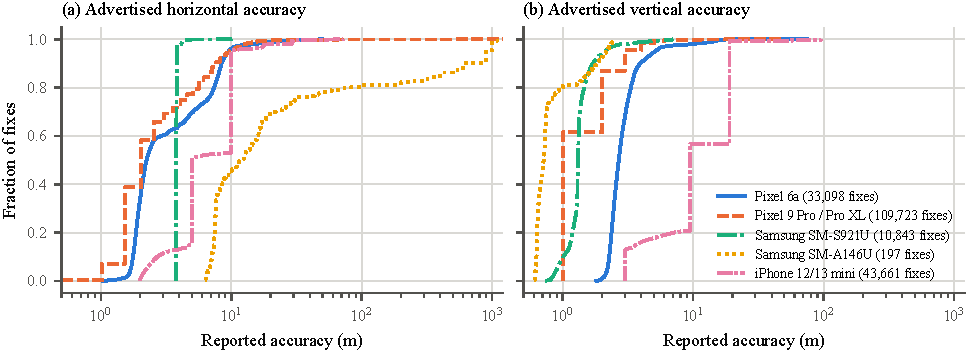
\includegraphics[width=\linewidth]{figures/fig_gnss_accuracy.pdf}
\caption{Empirical distribution of the horizontal (a) and vertical (b) accuracy reported with each GNSS fix in the processed trajectories, pooled by device family. Line styles distinguish families in addition to color.}
\label{fig:gnss}
\end{figure}

One trajectory is markedly worse than the rest. \texttt{2025-06-14\_21-17-02}, the only Samsung SM-A146U recording with data, delivered \numBadRawFixes{} location fixes in its raw file and \numBadFixes{} in the processed trajectory over \numBadSpan~s, a rate of \numBadFixRate{} fixes per second with gaps of up to \numBadMaxGap~s. Its median reported horizontal accuracy is \numBadHacc~m, and \numBadSentinels{} of its fixes report 999~m or more (up to \numBadHaccMax~m). It is kept in the release as a realistic poor-reception case. It dominates any aggregate that includes it, however (\Cref{sec:benchmark}), and users may prefer to report results with and without it.

\subsection{The operating-system gravity vector}
\label{sec:gravity}

The \texttt{Gravity} stream is not an accelerometer measurement. It is the operating system's fused estimate of the gravity direction, and its norm carries no information about local gravity. \Cref{fig:gravity} shows, for every raw sample, how far the norm falls below the largest norm in its recording. In \numGravRawPinnedRecordings{} of the \numUsedRecordings{} recordings that enter the processed set, every raw sample lies within 1~mGal (\(10^{-5}\)~m/s\(^2\)) of the recording's maximum. That maximum is a device constant: a median of \numGravPixel~m/s\(^2\) on the Pixel phones and \numGravSamsungApple~m/s\(^2\), standard gravity, on the Samsung SM-S921U and the iPhones. The exception, the Samsung SM-A146U, varies by tens of mGal below \numGravAfourteen~m/s\(^2\) (5th to 95th percentile of the deficit: \numGravAfourteenPfiveDeficit{} to \numGravAfourteenPninetyfiveDeficit~mGal). That variation is far larger than the gravity anomaly signal along these tracks. The 10~Hz bin averaging spreads the pinned norm slightly. In the processed files a median trajectory has \numGravTenHzPinnedMedian\% of its rows within 1~mGal of its maximum, which matches the figure reported by \citet{brodovsky2026dissertation}. Against the free-air anomaly map, the median per-trajectory signal-to-noise ratio of the resulting anomaly measurement is \numSnrGravity{} (best trajectory \numSnrGravityBest), below one on every trajectory \citep{brodovsky2026dissertation}. The \texttt{grav\_*} columns are useful as the operating system's attitude reference, not as a gravimeter.

\begin{figure}[t]
\centering
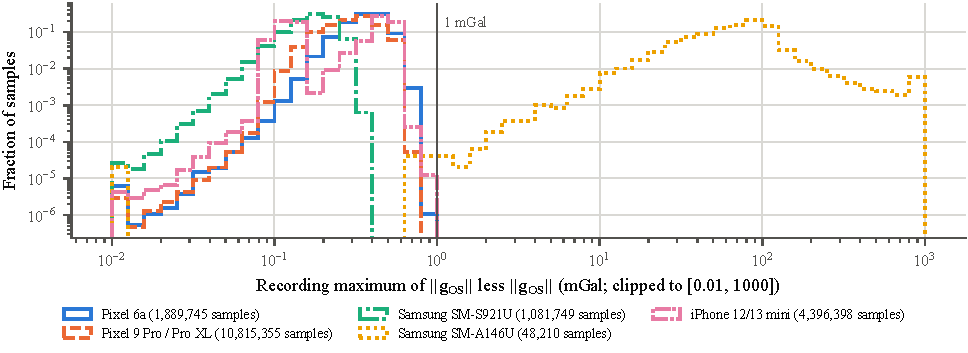
\includegraphics[width=\linewidth]{figures/fig_gravity_norm.pdf}
\caption{Norm of the operating-system gravity vector at the raw rate, expressed as its shortfall from the largest norm in the same recording and pooled by device family. Every family except the Samsung SM-A146U stays within 1~mGal (vertical line) of a fixed value throughout every recording.}
\label{fig:gravity}
\end{figure}

\subsection{The magnetometer}
\label{sec:magnetometer}

The \texttt{Magnetometer} stream is already hard-iron corrected by the operating system. In the \numHardIronCount{} processed recordings that also contain \texttt{MagnetometerUncalibrated}, the difference between the median uncalibrated and median calibrated field ranges from \numHardIronMin{} to \numHardIronMax~\(\mu\)T in magnitude. The calibrated field is still dominated by the vehicle. The median calibrated intensity of the processed trajectories ranges from \numMagIntensityMin{} to \numMagIntensityMax~\(\mu\)T, although all of them were recorded within a few hundred kilometres of each other and the geomagnetic field \citep{wmm} varies far less over that region. Fitting the heading-dependent pattern of the field leaves a body-fixed horizontal field of 56~\(\mu\)T at the median, larger than the Earth's horizontal field, and vehicle heading explains 57\% of the variance of the observed intensity \citep{brodovsky2026dissertation}. The median per-trajectory signal-to-noise ratio of the magnetic anomaly measurement against the WDMAM grid is \numSnrMagnetic{} (best \numSnrMagneticBest). The magnetometer direction can still support a heading measurement, but magnetic anomaly navigation from these phones would first need a vehicle calibration that the data do not provide.

\subsection{Replay, degradation and baselines}
\label{sec:benchmark}

Every processed trajectory can be replayed by the strapdown-rs simulator \citep{strapdown-rs}, which implements strapdown mechanization in the local-level frame after \citet{groves}. The recordings follow the east--north--up convention for specific force (\Cref{sec:processed}), so the simulator is run with \texttt{is\_enu = true}; it checks the declared frame against the data and refuses a mismatch. The simulator's GNSS degradation acts at two levels. A scheduler decides which recorded fixes the filter receives: all of them, one every fixed interval, or alternating on and off windows. A fault model then corrupts the delivered fixes, either with first-order autoregressive (AR(1)) noise on position and velocity together with inflated reported covariance \citep{wang2022noise}, with a slow drift, or with a step offset during a time window. Every random draw comes from a seeded generator, so a configuration file reproduces a run exactly.

The baselines in \Cref{tab:benchmark} use two scenarios. With \emph{full} GNSS, every recorded fix is delivered unmodified. With \emph{degraded} GNSS, one fix every 60~s is delivered. It carries AR(1) position error with a steady-state standard deviation of 35~m and a correlation time of 500~s, and AR(1) velocity error of 1.5~m/s with a correlation time of 100~s. The reported standard deviations are scaled by 5, so the measurement covariance grows by 25, and the seed is 42. Three filters were run: a loosely coupled extended Kalman filter (EKF), an unscented Kalman filter (UKF), and a Rao--Blackwellized particle filter (RBPF) after \citet{canciani2017airborne} \todo{confirm the particle count used for these runs; their configurations were not archived}. The simulator also passes the barometric relative altitude and a magnetometer-derived heading to the filters at its default schedule of one per second \todo{confirm which of these each filter consumed, and the strapdown-rs commit that produced the benchmark files}. No geophysical measurement was used. Performance is the horizontal great-circle distance between the filter's position and the recorded GNSS fix, evaluated at every recorded fix, including the fixes withheld from the filter. It is summarized per trajectory as a root-mean-square error (RMSE) and then across trajectories.

\begin{table}[t]
\centering
\caption{Reference baselines: horizontal RMSE against the recorded GNSS track, summarized over trajectories, and the median vertical RMSE. \(n\) is the number of trajectories on which the run completed. Errors of 10~km or more are given in kilometres.}
\label{tab:benchmark}
\small
\setlength{\tabcolsep}{4pt}
\begin{tabular}{llrrrrr}
\toprule
Filter & GNSS & \(n\) & Median (m) & Mean (m) & Max (m) & Vert.\ median (m) \\
\midrule
EKF & Full & 27 & 4.1 & 24.0 & 539.2 & 1.6 \\
 & Degraded & 27 & 440.4 & 611.4 & 2{,}436.1 & 23.4 \\
\midrule
UKF & Full & 27 & 4.0 & 24.0 & 542.8 & 1.6 \\
 & Degraded & 27 & 430.4 & 577.1 & 3{,}115.4 & 24.0 \\
\midrule
RBPF & Full & 27 & 1.9 & 181.7 & 3{,}628.5 & 1.6 \\
 & Degraded & 26 & 817.7~km & 941.9~km & 2{,}704.3~km & 445.7 \\
\bottomrule
\end{tabular}

\end{table}

With full GNSS, the EKF and UKF follow the recorded track to a median horizontal RMSE of \numEkfFullMedian{} and \numUkfFullMedian~m. On every trajectory except \texttt{2025-06-14\_21-17-02} the RMSE is at most \numEkfFullMaxOthers~m, while on that trajectory it is \numEkfFullBad~m (EKF) and \numUkfFullBad~m (UKF). This agreement mainly shows that the replay and the column conventions are consistent; it is not a measure of absolute accuracy (\Cref{sec:limitations}). With degraded GNSS, the median grows to \numEkfDegradedMedian~m (EKF) and \numUkfDegradedMedian~m (UKF). That is the regime in which an alternative aiding source has to prove itself, and the baseline that such a source should be compared against. The RBPF configuration that was used tracks well with full GNSS (median \numRbpfFullMedian~m), but it diverges in the degraded scenario: its median RMSE is \numRbpfDegradedMedian{} on the \numRbpfDegradedN{} trajectories that completed, and \numRbpfDegradedMissing{} did not complete. It is reported as a configuration that fails, not as a usable baseline. The scenario files and the per-trajectory results are included in the release (\Cref{sec:layout}).

\section{Limitations}
\label{sec:limitations}

\begin{itemize}
\item \textbf{No independent reference.} The reference trajectory is the phone's own GNSS solution, with the accuracies of \Cref{sec:gnss}. Nothing in the dataset measures position more accurately than that. Errors computed against it, including those in \Cref{tab:benchmark}, measure agreement with the recorded GNSS track, not absolute error. They are meaningful when the estimate under test is substantially worse than the GNSS, as in GNSS-outage and degradation studies, and lose meaning as the estimate approaches metre level. Attitude and velocity have no reference beyond the operating system's own estimates and the GNSS velocity.
\item \textbf{Unknown installation.} \todo{state what is known about phone placement.} Lever arms, mounting orientation and any movement of the phone within the vehicle were not recorded, and the body axes are the phone's, not the vehicle's.
\item \textbf{Opaque on-device processing.} The calibrated inertial streams, the gravity and attitude estimates, the hard-iron correction and the location fixes are all produced by proprietary operating-system and chipset software that differs between devices and changes with software updates. \Cref{sec:gravity,sec:magnetometer} show two consequences: the gravity norm is fixed at a constant, and the calibrated magnetic field still contains the vehicle's field.
\item \textbf{Uneven coverage.} One phone family, the Pixel 9 Pro, contributes 13 of the \numTrajectories{} trajectories. All drives are in one region of the north-eastern United States and most are on highways. Urban canyons, tunnels and genuinely jammed or spoofed GNSS are absent; degradation is simulated, not recorded.
\item \textbf{Platform differences.} Sampling rates differ between devices (\Cref{tab:channels}), iPhones deliver pressure at about 1~Hz, and GNSS comes from Android's GNSS-only provider on Pixel phones but from the fused location service elsewhere. Reported altitude is not consistent across platforms (\Cref{sec:gnss}).
\item \textbf{Processing choices.} The processed files are bin-averaged to 10~Hz and split at inertial dropouts. Two iPhone recordings without barometer data (\numNoBaroHours~h) appear only in the raw tier. The trajectory \texttt{2025-06-14\_21-17-02} has sparse, low-quality GNSS (\Cref{sec:gnss}).
\item \textbf{Baselines are reference points, not tuned results.} The filter configurations in \Cref{tab:benchmark} were not optimized per trajectory, and the RBPF configuration diverges under the degraded scenario.
\end{itemize}

\section*{Ethics statement}

The data were recorded by the authors and by volunteers driving on public roads. No human-subject experiment was performed and no data on third parties were collected. The recordings contain no audio, images or personal identifiers beyond the location traces themselves and an application-generated device identifier in \texttt{Metadata.csv}. \todo{confirm the volunteers' written consent to publication; confirm whether Temple University's IRB determined this not to be human-subjects research; decide whether to trim the start and end of each trace near private residences and whether to remove or replace the \texttt{device id} field before release.} The authors have read and follow the ethical requirements for publication in Data in Brief and confirm that the current work does not involve human subjects, animal experiments, or any data collected from social media platforms.

\section*{CRediT authorship contribution statement}

\textbf{James Brodovsky:} Conceptualization, Methodology, Software, Investigation, Data curation, Formal analysis, Visualization, Writing -- original draft. \textbf{Philip Dames:} Supervision, Writing -- review \& editing. \todo{confirm roles, including any funding acquisition.}

\section*{Acknowledgements}

The authors thank Beth Brodovsky, Jeremy Brodovsky, Monica Brodovsky, Bill Siegl and Alkesh Kumar Srivastava for their help in recording the drives. \todo{funding statement, or ``This research did not receive any specific grant from funding agencies in the public, commercial, or not-for-profit sectors.''}

\section*{Declaration of competing interests}

The authors declare that they have no known competing financial interests or personal relationships that could have appeared to influence the work reported in this paper. \todo{confirm.}


\bibliographystyle{elsarticle-harv}
\bibliography{references}

\end{document}
